\documentclass[9pt,conference]{IEEEtran}
\usepackage[utf8]{inputenc}
\usepackage[brazil]{babel}

% Diversos
\usepackage{csquotes}
\usepackage{graphicx}
\usepackage{verbatim}
\usepackage{hyperref}
\usepackage{smartdiagram}

% Título
\title{Utilizando Redes Convolucionais de Grafos Espaço-Temporais para o Reconhecimento da Línguas de Sinais}
%\author{Cleison Correia de Amorim}
\date{Outubro 2018}

\author{
    \IEEEauthorblockN{Cleison Correia de Amorim}
    \IEEEauthorblockA{Centro de Informática\\
    Universidade Federal de Pernambuco\\
    Email: cca5@cin.ufpe.br}
}

% Comandos
% 'image': definição de imagem
\newcommand{\image}[4][\linewidth] {
    \begin{figure}[ht]
    \centering
    \includegraphics[width=#1]{#3}
    \caption{#4}
    \label{#2}
    \end{figure}
}

% 'refimage': referências de imagens
\newcommand{\refimage}[1] {figura \ref{#1}}

% 'refsection': referências de seções
\newcommand{\refsect}[1] {seção "\nameref{#1}"}

\begin{document}
\maketitle
\begin{abstract}
Este trabalho propõe a aplicação de um modelo de aprendizagem profunda baseado em grafos, conhecido como Rede Convolucional de Grafos Espaço-Temporais, para o reconhecimento de sinais da língua sinalizada. Trata-se de uma abordagem centrada no movimento do corpo humano, o qual é capturado no espaço e no tempo e representado na forma de grafos, que são posteriormente aprendidos automaticamente pelo modelo.
\end{abstract}

%\begin{IEEEkeywords}
%Broad band networks, quality of service, WDM.
%\end{IEEEkeywords}


\section{Introdução} %%%%%%%%%%%%%%%%%%%%%%%%%%%%%%%%%%%%%%%%%%%
\label{sec:introducao}
[TODO: incluir introdução sobre a língua da sinais...]

Hoje há um grande número de estudos que se propõem realizar a transcrição da língua de sinais para sua equivalência na língua falada. Entretanto, muitos desses estudos apresentam-se limitados frente ao cotidiano do Surdo por desconsiderarem aspectos relevantes da fonologia dessa língua como, por exemplo, movimentos, expressões não-manuais e locação (ou pontos de articulação) \cite{quadros-2004} e abordam o problema utilizando imagens estáticas dos sinais ou restringindo seu foco apenas às mãos do interlocutor sem a interação com o próprio corpo. É comum também que tais estudos centralizem seu campo de atuação ao âmbito da datilologia\footnote{
     Datilologia – também conhecida como alfabeto digital ou alfabeto manual. Consiste na soletração de palavras pelos Surdos. É geralmente utilizada para introduzir uma palavra que ainda não possui um sinal equivalente \cite{quadros-2004, pereira-choi-2011}.
}, que na prática é aplicada apenas em contexto restritos da comunicação desses indivíduos.

Em \cite{antunes-hcisl-2011}, os autores reiteram os fatores acima e adicionam outros que expõem a dificuldade em trazer esse tipo de estudos para a realidade do Surdo: 
\begin{enumerate}
    \item O uso de equipamentos como luvas, acelerômetros e outros sensores que são de difícil acesso; 
    \item A adoção de métodos e tecnologias que não empatizam com a realidade Surdo, restringindo sua movimentação ou deixando de considerar características importantes, como as expressões faciais;
    \item O uso de métodos que mapeiam sinais diretamente para palavras, e que tornam-se facilmente obsoletos mediante a introdução de novos sinais ou quando confrontados com variações linguísticas como gírias e regionalismos; 
    \item A utilização de imagens estáticas para o treinamento de modelos, que desconsideram a dinâmica da língua.
\end{enumerate}

Diante dessas limitações, é apresentada em \cite{antunes-hcisl-2011} e \cite{garcia-2013} uma arquitetura denominada HCI-SL, que tem como proposta considerar aspectos fonológicos da língua para viabilizar a interação entre homem e máquina por meio de sinais. A \refimage{fig:hcisl} apresenta a arquitetura em mais detalhes. É possível observar que as técnicas e ferramentas de inteligência computacional exercem um papel essencial nas camadas mais básicas da estrutura proposta, e compreendem atuam a ponta da interação do interlocutor para com a máquina.

\image
	[5cm]
    {fig:hcisl}
    {images/hcisl}
    {Arquitetura HCI-SL, composta por uma API interna contendo tecnologias de visão e inteligência computacional e uma camada de \textit{frameworks} que provê uma interface padrão para ferramentas e serviços externos como dicionários, tradutores e aplicativo de fins diversos. Fonte: \cite{antunes-hcisl-2011}.}

Para que essa arquitetura funcionasse, era também necessário definir uma forma homogênea de representar os sinais, que viria a ser utlizada pelas camadas internas e os serviços externos que consumissem a interface provida pela estrutura. Dessa forma, introduziu-se em \cite{antunes-2011} e \cite{antunes-2015} uma representação denominada por CORE-SL, que baseia-se nas características fonológicas da língua de sinais para descrevê-los computacionalmente. Segundo os autores, essa representação agrega flexibilidade e um nível de detalhamento capazes de proporcionar alternativas para um tratamento computacional robusto e para auxiliar às diferentes necessidades de aplicação. 

Dado o contexto acima, esta pesquisa objetiva contribuir com a viabilização da arquitetura HCI-SL sob a dimensão das técnicas de inteligência computacional necessárias para compor sua base fundamental, bem como com a proposição de caminhos que contornem os problemas apontados nas abordagens apresentadas anteriormente quando confrontadas com o cotidiano do Surdo. 

O primeiro passo nessa direção consiste em quebrar a barreira da representação estática dos sinais para identificar e explorar abordagens capazes de considerar os traços do movimento do corpo do interlocutor, bem como a interação entre suas partes e as expressões decorrentes da articulação dos sinais. Para isso, nas seções a seguir será apresentada e avaliada a eficácia da aplicação de uma técnica de aprendizagem profunda denominada Rede Convolucional de Grafos Espaço-Temporais \cite{st-gcn-2018}, que é centrada nos movimentos do corpo, mãos e face do interlocutor capturados por meio de câmeras convencionais e representados como grafos, para o reconhecimento de sinais. 


\section{Trabalhos Relacionados} %%%%%%%%%%%%%%%%%%%%%%%%%%%%%%%%%%%%%%%%%%%

[TODO: incluir conteúdo]


\section{Redes Convolucionais de Grafos Espaço-Temporais} %%%%%%%%%%%%%%%%%%%%%%%%%%%%%%%%%%%%%%%%%%%

As Redes Convolucionais de Grafos Espaço-Temporais (ou \textit{Spatial-Temporal Graph Convolutional Network - ST-GCN}) consistem num tipo de modelo de aprendizagem profunda proposto por \cite{st-gcn-2018} que especializa a abordagem das Redes Neurais de Grafos e que são aplicados no reconhecimento de ações. Sua motivação surgiu a partir da necessidade enxergada pelos autores de métodos que fossem capazes de capturar de forma autônoma os padrões contidos na configuração espacial das articulações do corpo humano, bem como sua dinâmica temporal.

Segundo os autores, métodos anteriores de uso de esqueletos para reconhecimento de ações acabaram limitando-se justamente por não explorar explicitamente tais relações espaciais entre as articulações, que são cruciais para a compreensão das ações humanas. Esses métodos, simplesmente empregaram as coordenadas conjuntas em etapas de tempo individuais para formar vetores de característica, aplicando uma análise temporal neles \cite{st-gcn-2018, wang-2012, fernando-2015}.

%A capacidade desses métodos é limitada, pois eles não exploram explicitamente as relações espaciais entre as articulações, que são cruciais para a compreensão das ações humanas.

Mais recentemente, novos métodos que tentaram alavancar as conexões naturais entre as articulações foram desenvolvidos \cite{shahroudy-2016, yong-du-2015}. Eles mostraram melhorias encorajadoras, o que sugere a importância da conectividade. No entanto, a maioria desses métodos baseia-se em partes ou regras criadas manualmente para analisar os padrões espaciais. Como resultado, os modelos criados para uma aplicação específica são difíceis de serem generalizados para outras \cite{st-gcn-2018}.

O ST-GCN, por sua vez, tem como base de sua formulação a sequência de grafos de esqueletos que representam o corpo humano, os quais são obtidos a partir de uma sequência de frames de vídeos de ações ordinárias desses indivíduos. A \refimage{fig:st-gcn-graph} permite-nos visualizar essa estrutura, onde cada nó corresponde a um ponto de articulação humana. Os vértices intra-corporais são definidos com base nas conexões naturais do corpo. Os vértices inter-frames, por sua vez, conectam as mesmas conexões (ou articulações) entre frames consecutivos para denotar sua trajetória no decorrer do tempo \cite{st-gcn-2018}.

\image
	[4cm]
    {fig:st-gcn-graph}
    {images/st_gcn_graph}
    {Sequência de grafos de esqueletos, que denotam o movimento humano no espaço e no tempo, utilizados pelo ST-GCN. Fonte: \cite[p. 1]{st-gcn-2018}.}

A \refimage{fig:st-gcn-workflow} ilustra a abordagem utilizada pelo ST-GCN. Em primeiro lugar, é realizada a estimação das poses dos indivíduos nos vídeos de entrada e a construção de grafos espaço-temporais com base na sequência de esqueletos estimados. Em seguida, múltiplas camadas de convolução ST-GCN são aplicadas gerando, gradualmente, mapas de características de nível cada vez mais alto para os grafos apresentados. Por fim, eles são submetidos a um classificador para a identificação da ação correspondente.

\image
    {fig:st-gcn-workflow}
    {images/st_gcn_workflow}
    {Fluxo do ST-GCN, onde os grafos criados a partir dos indivíduos presentes nos vídeos são submetidos ao modelo e, por fim, classificados entre as ações disponíveis. Fonte: \cite[p. 3]{st-gcn-2018}.}


% Funcionamento do ST-GCN ------------------------

Para que seja possível compreender o funcionamento da rede ST-GCN, é necessário primeiro aprofundarmos a discussão nas estratégias de amostragem e de particionamento adotadas pelos autores. 

Quando lidamos com convoluções em imagens 2D, facilmente visualizamos a existência de um \textit{grid} rígido ou retângulo em volta de um ponto central, o qual delimita a vizinhança na qual o filtro convolucional será aplicado. No caso dos grafos, entretanto, é necessário ir além dessa definição e considerar que a vizinhança de um ponto será composta apenas por aqueles pontos que estão diretamente conectados a ele por meio de uma borda. A \refimage{fig:st-gcn-sampling} permite-nos visualizar essa definição para o exemplo de um único \textit{frame}. Observe que as bordas tracejadas vermelhas passam a representar a área de amostragem utilizada pelo filtro convolucional, em volta dos pontos centrais em vermelho. Observe também que, apesar de haver pontos do corpo localizados próximos fisicamente no espaço (como nos pontos dos pés, joelhos e cintura), eles não serão considerados como vizinhos na abordagem de convolução em grafos por não possuírem conexões diretas entre si.

\image
	[3cm]
    {fig:st-gcn-sampling}
    {images/st_gcn_sampling}
    {\textit{Frame} de exemplo de um esqueleto de entrada. As articulações do corpo são desenhadas com pontos azuis. Os pontos vermelhos representam os pontos centrais de um filtro com distância D = 1 aplicado ao \textit{frame}, cuja abrangência é delimitada pela linha tracejada vermelha. Fonte: \cite[p. 5]{st-gcn-2018}.}

Por meio da \refimage{fig:st-gcn-sampling} é possível observar que apenas estão sendo considerados pela linha tracejada os pontos que estão imediatamente conectados aos pontos centrais. Em outras palavras, diz-se que a área de amostragem do filtro convolucional apenas considera vizinhos com distância D = 1. Essa distância poderia ser ajustada para abranger vizinhos mais distantes, porém na apresentação do ST-GCN \cite{st-gcn-2018} os autores estabeleceram a utilização da distância conforme acima.

Uma vez apresentada a estratégia de amostragem, é possível seguir na compreensão da estratégia de particionamento utilizada pelo ST-GCN. Ela é definida como Particionamento de Configuração Espacial e baseia-se na localização das partes do corpo humano e nas características de seu movimento, conforme ilustra a \refimage{fig:st-gcn-spatial-part}.

\image
	[3cm]
    {fig:st-gcn-spatial-part}
    {images/st_gcn_spatial_partitioning}
    {Particionamento de Configuração Espacial: os nós são rotulados de acordo com suas distâncias ao centro de gravidade do esqueleto (cruz preta) comparado com o do nó raiz (verde). Os nós centrípetos têm distâncias menores (azul), enquanto os nós centrífugos têm distâncias mais longas (amarelo) do que o nó raiz. Fonte: \cite[p. 5]{st-gcn-2018}.}

De acordo com os autores, a estratégia desenvolvida motiva-se no fato de que os movimentos das partes do corpo podem ser amplamente categorizados como concêntricos ou excêntricos e, por isso, particiona a vizinhança em três subconjuntos:

\begin{enumerate}
    \item O nó raiz (ou ponto central, sinalizado em verde na imagem);
    \item O grupo centripetal (pontos em azul na imagem): nós da vizinhança que estão mais próximos do centro de gravidade do esqueleto (cruz preta na imagem) do que o nó raiz;
    \item O grupo centrifugal (pontos em amarelo na imagem): mais distante do centro de gravidade do que o nó raiz;
\end{enumerate}

O centro de gravidade é tomado como sendo a coordenada média de todas as juntas do esqueleto em um \textit{frame} e, durante a convolução, cada ponto do corpo é rotulado segundo uma das partições acima.

O ST-GCN define uma estratégia de atribuição de pesos que também é direcionada pelas partições acima e, para cada uma delas, atribui um peso distinto. Isso é um detalhe importante sobre o modelo que, ao invés de concentrar sua atenção no movimento das juntas do corpo de forma individual,  direciona seu foco a aprender o tipo do movimento realizado por essas juntas.

Uma vez exploradas as estratégias definidas pelo ST-GCN, apresentadas sob o contexto de um único \textit{frame} na dimensão espacial, podemos dar um passo adiante para compreender como o modelo considera a dimensão temporal. 

Primeiramente, retomemos à definição inicial que estabelece que a dimensão temporal é representada por uma sequência de grafos extraídos dos \textit{frames} de vídeo da ação de um indivíduo, conforme ilustrado na \refimage{fig:st-gcn-graph}. Se selecionarmos o grafo de um \textit{frame} aleatório nessa sequência, podemos considerar que ele possui dois vizinhos: aquele imediatamente anterior e aquele imediatamente posterior a ele na sequência. Além disso, foi definido também que cada junta do corpo em um grafo precisar estar conectada a ela mesma nos grafos vizinhos para representar sua evolução no tempo.

Se considerarmos o racional acima, e nos voltarmos para a definição de amostragem representada na \refimage{fig:st-gcn-sampling} é fácil evoluir a compreensão espacial para a dimensão temporal quando consideramos que o ponto central em vermelho, além dos pontos delimitados pela linha tracejada vermelha, passará a ter como vizinhos também aqueles pontos com os quais está conectado nos grafos vizinhos dos \textit{frames} anterior e posterior da sequência. Dessa forma, a linha tracejada vermelha passará a englobar mais pontos dentro dela, abrangendo agora também aqueles diretamente conectados e dispostos na dimensão temporal, conforme ilustrado na \refimage{fig:st-gcn-convolution} (à esquerda).

\image
	[9cm]
    {fig:st-gcn-convolution}
    {images/st_gcn_convolution}
    {Amostragem englobando pontos diretamente conectados nas dimensões espacial e temporal (à esquerda) e processo de convolução espaço-temporal sob os pontos da amostragem obtida (ao centro e à direita).  Fonte: \cite[p. 3]{st-gcn-2018}.}

Uma vez realizada a amostragem sob ambas as dimensões e selecionados os pontos para aplicação da convolução, é possível aplicar esse processo de uma forma análoga àquela aplicada a imagens 2D, conforme ilustra a \refimage{fig:st-gcn-convolution} (ao centro e à direita).


% Arquitetura ------------------------

A \refimage{fig:st-gcn-architecture} (à esquerda) permite-nos visualizar as camadas de convolução do modelo. Ao todo, são nove camadas convolucionais ST-GCN posicionadas de forma sequencial, que realizam a extração das características dos grafos espaço-temporais apresentados. Elas são precedidas por uma camada de normalização e seguidas por uma camada de \textit{pooling} global e outra de classificação \textit{softmax}. À direita da imagem é apresentado também o detalhe de uma unidade convolucional ST-GCN.

\begin{figure}[ht]
    \centering
    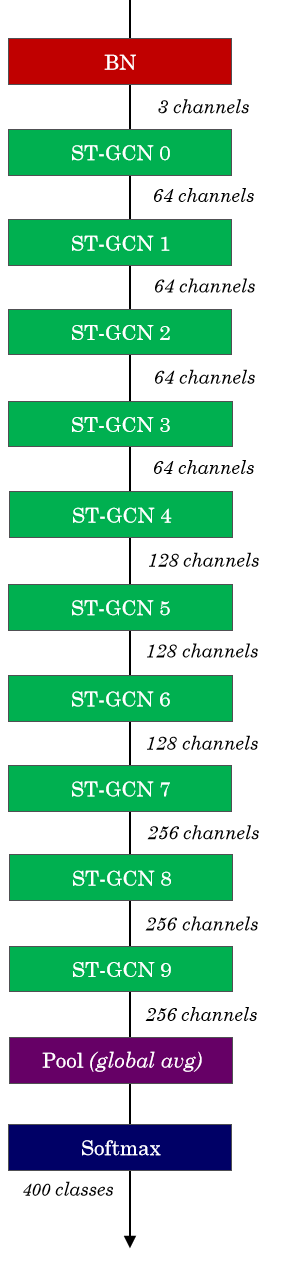
\includegraphics[width=3.0cm]{images/st_gcn_architecture}
    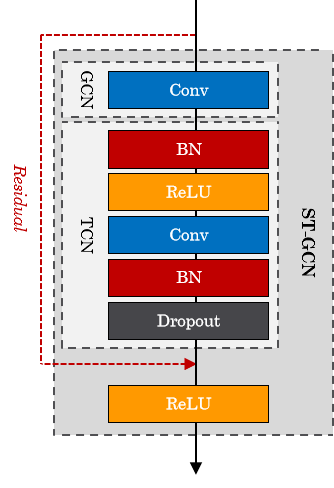
\includegraphics[width=3.5cm]{images/st_gcn_architeture_unit}
    \caption{Arquitetura do modelo (à esquerda) e detalhe de uma unidade ST-GCN (à direita). Unidades de ST-GCN aplicam operações de normalização, convolução, ativação e \textit{dropout} aos grafos e levam em consideração o valor residual da camada anterior para calcular as ativações de saída. Fonte: adaptado de \cite{st-gcn-2018}.}
    \label{fig:st-gcn-architecture}
\end{figure}


Para que fosse possível realizar a estimação das poses dos indivíduos, conforme fluxo da \refimage{fig:st-gcn-workflow}, os autores utilizaram uma biblioteca denominada OpenPose. Trata-se de uma biblioteca que utiliza algoritmos de aprendizagem profunda para detectar indivíduos em cenas de vídeos e extrair até 135 pontos de articulações de seus corpos, mãos e faces \cite{cao-realtime-2017, simon-hand-2017, wei-cpm-2016}, e que está disponível publicamente\footnote{
    Disponível em \url{https://github.com/CMU-Perceptual-Computing-Lab/openpose}.
}.

Para apresentação do ST-GCN, entretanto, os autores utilizaram apenas 18 desses pontos, os quais se referem às articulações do corpo (vide \refimage{fig:keypoints-pose}). O código fonte e os modelos pré-treinados do ST-GCN estão disponíveis publicamente pelos autores\footnote{
    Disponível em \url{https://github.com/yysijie/st-gcn}.
}.

\image
	[4cm]
    {fig:keypoints-pose}
    {images/keypoints_pose_COCO_18}
    {Representação dos 18 pontos referentes ao corpo humano, extraídos pelo OpenPose. Fonte: \cite{openpose-output-2018}.}




\section{American Sign Language Lexicon Video Dataset} %%%%%%%%%%%%%%%%%%%%%%%%%%%%%%%%%%%%%%%%%%%

O \textit{American Sign Language Lexicon Video Dataset} (ou ASLLVD) consiste num \textit{dataset} público\footnote{
    Disponível em \url{http://csr.bu.edu/asl/asllvd/annotate/index.html}.
} amplo e em expansão que contém sequências de vídeos de milhares de sinais distintos da Língua Americana de Sinais (\textit{American Sign Language}, ou ASL), bem como as anotações dessas sequências, os \textit{frames} de início e fim, e os rótulos de classe para cada sinal \cite{athitsos-asllvd-2008, neidle-2012, vloger-2012}.

Segundo os autores, cada sinal é articulado por indivíduos nativos da ASL, e as sequências de vídeo são coletadas utilizando um sistema de quatro câmeras que captura simultaneamente duas vistas frontais, uma vista lateral e uma vista ampliada na face desses indivíduos. A \refimage{fig:asllvd-example} exemplifica a captura de três dessas vistas para o sinal "\textit{MERRY-GO-ROUND}".

\image
    {fig:asllvd-example}
    {images/asllvd_example}
    {Exemplo de captura do sinal \textit{"MERRY-GO-ROUND"} sob três perspectivas, no ASLLVD. Fonte:  \cite[p. 2]{athitsos-asllvd-2008}.}

Ainda de acordo com os autores, o número e o tipo de sinais incluídos no ASLLVD são semelhantes em escala e escopo ao conjunto de entradas lexicais nos dicionários existentes de "Inglês-para-ASL". Existe ao menos um exemplo de vídeo por sinal (articulado por um indivíduo nativo), para quase todos os sinais contidos no Dicionário Gallaudet de Língua Americana de Sinais \cite{athitsos-asllvd-2008, gallaudet-2005}. 

Ao analisar os metadados do \textit{dataset} é possível identificar a existência de um total de 2.745 sinais, representados em 9.757 amostras. Cada sinal contém entre 1 e 18 amostras articuladas por diferentes indivíduos (sendo 4 o número médio de amostras por sinal).


\section{Método de Pesquisa} %%%%%%%%%%%%%%%%%%%%%%%%%%%%%%%%%%%%%%%%%%%%%%%%%%%%%%%%%%%%%%%%%%%%%%%

A pesquisa foi organizada segundo passos estabelecidos abaixo. Em termos gerais, eles definem desde a identificação de um modelo em potencial conforme objetivos estabelecidos na \refsect{sec:introducao}, sua adaptação para o problema da língua de sinais até a avaliação de seu desempenho.

\begin{enumerate}
    \item Definir modelo: nesse passo foi selecionado o modelo ST-GCN e sua abordagem baseada em grafos para lidar com o problema da língua de sinais;
    \item Definir \textit{dataset}: foi estabelecido o ASLLVD, devido à sua abrangência relevante de sinais, qualidade das amostras coletadas, organização das anotações e rotulações, e articulação dos sinais por indivíduos nativos. Apesar de baseado na Língua Americana de Sinais, a utilização desse \textit{dataset} não restringe a abordagem apresentada à língua daquele país. Ao contrário, entende-se que é possível adotar o mesmo método a \textit{datasets} de línguas de outros países;
    \item Preparar \textit{dataset}: para que fosse possível utilizar o \textit{dataset} acima com o modelo ST-GCN foi necessário primeiro criar um \textit{pipeline} de pré-processamento, conforme descrito mais adiante nesta seção, afim de colocar cada amostra em  um formato compatível com a entrada do modelo;
    \item Adaptar modelo: para que fosse possível utilizar o ST-GCN no contexto da língua de sinais, foi necessário adaptá-lo às particularidades do problema. Dentre elas, a principal diz respeito à mudança na representação da dimensão espacial dos grafos, que passa a considerar não apenas os 18 pontos utilizados em \cite{st-gcn-2018}, mas também os 21 pontos de cada mão e os 70 pontos da face, conforme ilustrado na \refimage{fig:keypoints-face-hand}. Dessa forma, os grafos do modelo passaram a considerar um total de 130 pontos do corpo humano e suas relações;
    \item Treinar modelo adaptado: nesse passo, o modelo acima será submetido às amostras do \textit{dataset} para que possa desenvolver um conhecimento acerca do problema;
    \item Avaliar e melhorar resultados: a partir das descobertas obtidas na tarefa acima, serão realizados os eventuais ajustes no modelo, \textit{dataset} ou nas configurações do treinamento, e repetido o passo anterior.
\end{enumerate}


Para tornar as amostras do ASLLVD compatíveis com a entrada esperada pelo modelo ST-GCN foram aplicadas várias etapas de pré-processamento em série, as quais estão apresentadas na \refimage{fig:preprocessamento} e definidas em detalhe a seguir.

%\begin{figure}[ht]
%    \centering
%    \smartdiagramset{
%        border color=none,
%        back arrow disabled=true,
%        text width=1cm}
%    \smartdiagram[sequence diagram]{
%        Obter vídeos,
%        Segmentar amostras,
%        Estimar poses, 
%        Holdout, 
%        Processar amostras}
%    \caption{Etapas de pré-processamento aplicadas ao \textit{dataset} ASLLVD.}
%    \label{fig:preprocessamento}
%\end{figure}

\image
    {fig:preprocessamento}
    {images/dataset_preprocessing}
    {Etapas de pré-processamento aplicadas ao \textit{dataset} ASLLVD.}

A primeira delas consiste num passo preliminar de \textbf{obtenção dos vídeos} que compõem o \textit{dataset}, para reconstitui-lo localmente de forma automática e viabilizar as etapas posteriores. A relação das vídeos e respectivas seções contidas no ASLLVD, e que foi utilizada para guiar a sua reconstituição, está disponibilizada juntamente com ele em um arquivo de metadados específico\footnote{
    Disponível em \url{http://www.bu.edu/asllrp/dai-asllvd-BU_glossing_with_variations_HS_information-extended-urls-RU.xlsx}
}. Apesar do \textit{dataset} disponibilizar capturas de até 4 câmeras diferentes para um mesmo sinal, para este trabalho foi considerada apenas a captura realizada pela câmera frontal, que contepmla os movimentos do tronco, mãos e face, simultaneamente.

A etapa seguinte consiste em \textbf{segmentar os vídeos} obtidos, uma vez que cada um deles corresponde a uma seção contendo inúmeros sinais por indivíduo. O intuito dessa tarefa é constituir um novo conjunto organizado de forma tal que cada sinal esteja contido em um arquivo próprio, com seu respectivo rótulo. Para isso, também foi considerado o arquivo de metadados comentado acima, que dispõe dos rótulos aqui requeridos e das respectivas marcações de \textit{frames} de início e término para cada sinal nas seções. Como saída dessa etapa, são obtidos vídeos com duração média de 1 a 5 segundos e com aspecto semelhante ao que ilustra a \refimage{fig:sign-original}.

\image
    [6cm]
    {fig:sign-original}
    {images/sign_original}
    {Representação do sinal "EXAGGERATE", segmentado a partir das seções gravadas para o ASLLVD. Fonte: \cite{athitsos-asllvd-2008}.}

O terceiro passo consiste em \textbf{estimar as poses} dos indivíduos presentes nos vídeos segmentados. Para isso, foi utilizada a mesma abordagem adotada pelos autores em \cite{st-gcn-2018}, a qual consiste em aplicar o OpenPose para extrair as coordenadas do corpo desses indivíduos. Neste trabalho, entretanto, para que fosse possível abranger também as mãos e face, além daquelas referentes ao tronco, um número consideravelmente maior de coordenadas foi solicitada ao OpenPose. No total são 130 pontos, dos quais 21 pontos correspondem a cada uma das mãos; 70 pontos correspondem às coordenadas da face; e 18 correspondem aos pontos do tronco ou corpo (vide \refimage{fig:keypoints-face-hand} e \refimage{fig:keypoints-pose}). A saída da estimação pelo OpenPose consiste em múltiplos arquivos, um por \textit{frame}, no formato JSON contendo as coordenadas solicitadas e o nível de confiança para cada uma delas. Ao término dessa etapa, entretanto, todos esses arquivos são concatenados em um único arquivo JSON que contempla as coordenadas estimadas para toda a sequência de \textit{frames} do vídeo atual. A \refimage{fig:sign-pose} ilustra a reconstrução dessas coordenadas em uma imagem para o sinal "EXAGGERATE", exibido anteriormente. A \refimage{fig:sign-pose}, por sua vez, ilustra a mesma reconstrução sobreposta sobre o vídeo original.

\begin{figure}[ht]
    \centering
    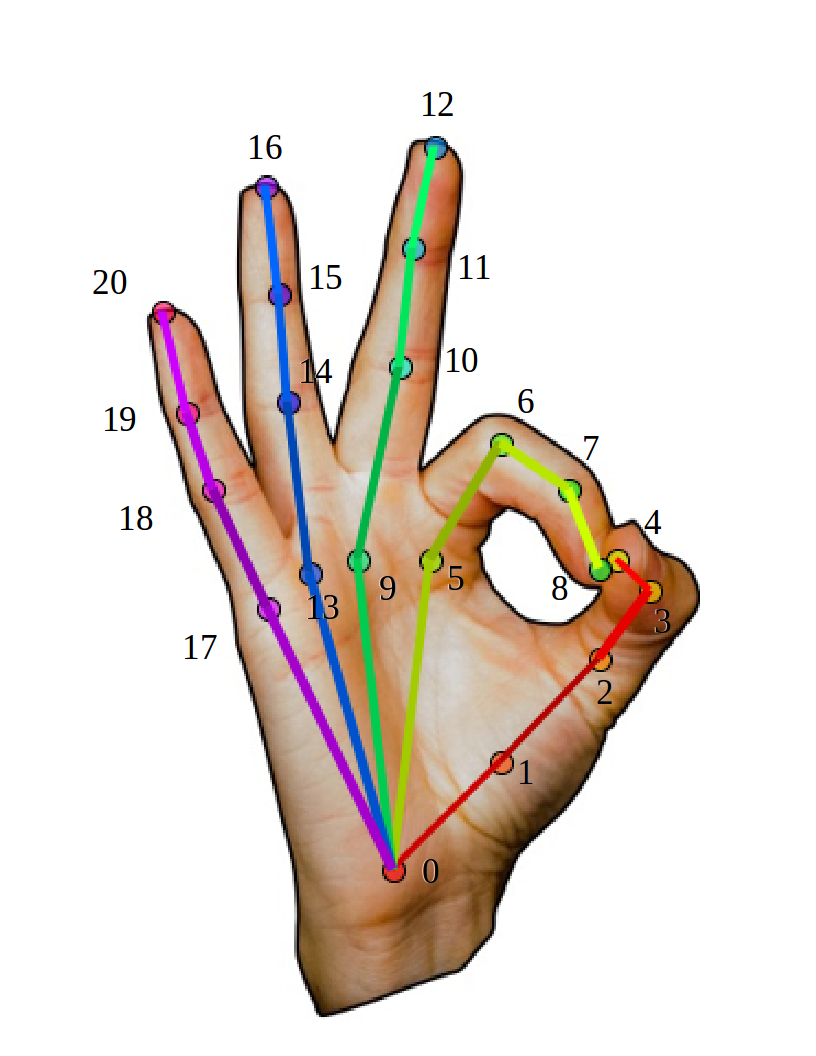
\includegraphics[width=3cm]{images/keypoints_hand}
    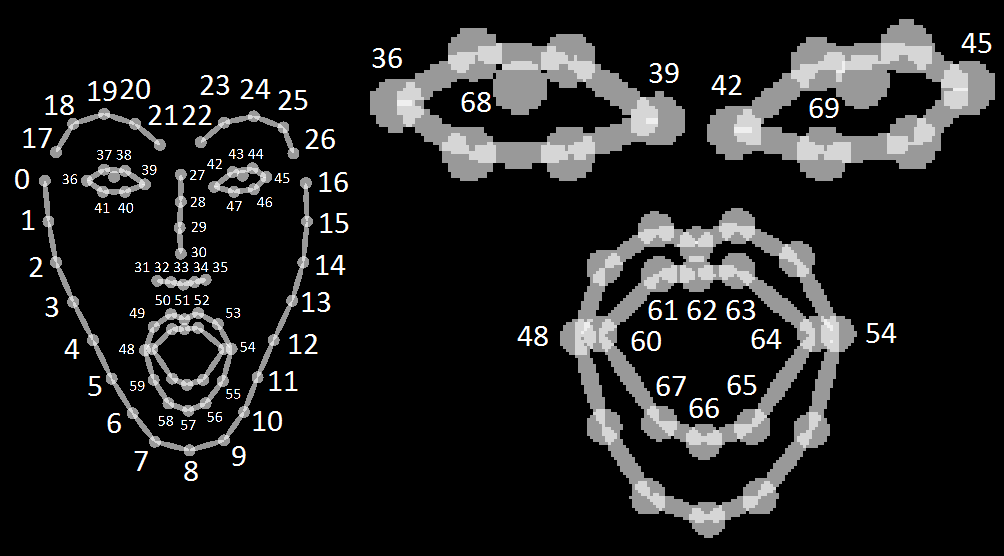
\includegraphics[width=5cm]{images/keypoints_face}
    \caption{Representação dos 21 pontos da mão (à esquerda) e 70 pontos da face (à direita), extraídos pelo OpenPose. Fonte: \cite{openpose-output-2018}.}
    \label{fig:keypoints-face-hand}
\end{figure}

\image
    [6cm]
    {fig:sign-pose}
    {images/sign_pose}
    {Reconstrução das coordenadas estimadas pelo OpenPose para o sinal "EXAGGERATE". Fonte: OpenPose.}

\image
    [6cm]
    {fig:sign-pose-blended}
    {images/sign_pose_blended}
    {Sobreposição das coordenadas estimadas pelo OpenPose no vídeo original para o sinal "EXAGGERATE". Fonte: adaptado de \cite{athitsos-asllvd-2008}.}

O passo posterior refere-se à \textbf{divisão do \textit{dataset}} nos subconjuntos de treinamento, testes e validação. 
% TODO: falar da biblioteca so scikit-learn utilizada


\begin{enumerate}
    %\item Obter vídeos: o \textit{dataset} está disponibilizado para download no formato de vídeos correspondentes a cada uma das seções gravadas, %conforme descrito no arquivo de metadados\footnote{
    %    Disponível em \url{http://www.bu.edu/asllrp/dai-asllvd-BU_glossing_with_variations_HS_information-extended-urls-RU.xlsx}
    %}. Os vídeos totalizam 126GB distribuídos em 952 arquivos. Para automatizar a obtenção desses itens, foi adicionado esse passo ao  \textit{pipeline} de pré-processamento;
    %\item Segmentar vídeos: como os vídeos do \textit{dataset} correspondem a seções inteiras gravadas para um indivíduo, que contém uma sequência de articulação de múltiplos sinais, faz-se necessário segmentar e rotular cada um deles em um arquivo próprio. Para isso, são utilizadas as anotações estabelecidas no arquivo de metadados;
    %\item Estimar poses: em seguida, é necessário utilizar a biblioteca OpenPose para extrair os 130 pontos do corpo dos indivíduos nas amostras. Esses pontos são extraídos para cada \textit{frame} e posteriormente são agrupados em um único arquivo JSON referente àquela amostra;
    \item Dividir \textit{dataset}: nessa etapa, as amostras devem ser separadas em subgrupos de treinamento, validação e testes. Para isso, foi utilizada uma proporção de 70\% dos dados para treinamento (cerca de 6.800 amostras), 15\% dos dados para validação (cerca de 1.500 amostras) e 15\% para testes (também cerca 1.500 amostras);
    \item Processar amostras: a implementação do modelo ST-GCN utiliza como formato de entrada listas de objetos do Python serializados e gravados no formato de arquivos \textit{.pkl}. Sendo assim, esse processo precisa ser aplicado aos conjuntos de amostras de treinamento, validação e testes divididos acima para o novo \textit{dataset}. Além disso, nessa etapa as amostras também deverão ser ajustadas para possuir um comprimento uniforme. Para isso, a sequência de \textit{frames} de cada amostra deve ser repetida preenchendo os \textit{frames} vazios até que o comprimento desejado seja alcançado, conforme sugerem os autores em \cite{st-gcn-2018}. Neste trabalho, um comprimento fixo de 126 \textit{frames} será adotado para as amostras (aproximadamente 4 segundos, considerando uma taxa de 30 FPS).
\end{enumerate}




\section{Resultados} %%%%%%%%%%%%%%%%%%%%%%%%%%%%%%%%%%%%%%%%%%%
\label{sec:resultados}

Esta seção apresenta as descobertas e resultados obtidos a partir da aplicação da abordagem descrita nas seções anteriores. Os experimentos aqui relacionados foram realizados utilizando uma máquina virtual com CPU Intel Haswell, memória RAM de 5GB e GPU NVIDIA Tesla P100 com 16GB de memória dedicada. O tempo médio obtido com essa arquitetura foi de aproximadamente 7 épocas para cada hora de treinamento.
% O tempo médio consumido para essa tarefa é proporcional ao número de épocas configuradas e tem variado entre 1 e 4 dia

Foram considerados \textit{batches} de 32 amostras e uma taxa de aprendizado de 0,1, além de um \textit{weight decay} de 0,0001 em quatro momentos distintos do treinamento (geralmente distribuídos após a conclusão de 35\%, 50\%, 65\% e 80\% das épocas previstas, respectivamente). 
Adicionalmente, uma estratégia de \textit{data augmentation} para diversificar as amostras apresentadas ao modelo, e ela consiste na aplicação de transformações randômicas de rotação, translação e escala no momento da leitura desses itens nos \textit{batches}.

A \reftable{tab:resultados-1} apresenta os resultados parciais obtidos da abordagem proposta neste trabalho (representado como ST-GCN (Sign Language), e aqueles obtidos pelo modelo ST-GCN em \cite{st-gcn-2018} (para os \textit{datasets} Kinetics e Kinetics Motion). O resultado do ST-GCN (Sign Language) está listado para o seu treinamento até a época 630 de um total de 1.000 previstas.

\begin{table}[ht]
    \centering
    \caption{Performance atual da abordagem proposta e do ST-GCN original}
    \label{tab:resultados-1}
    \begin{tabular}{@{}lll@{}} \toprule
                                        &   Top-1           &   Top-5           \\ \midrule
        ST-GCN (Kinetics)               &   30,7\%          &   52,8\%          \\
        ST-GCN (Kinetics Motion)        &   72,4\%          &   -               \\ \midrule
        \textbf{ST-GCN (Sign Language)} & \textbf{26,0\%}   &   \textbf{45,2\%} \\ \bottomrule
    \end{tabular}
\end{table}

De acordo com os autores em \cite{st-gcn-2018}, os \textit{datasets} Kinetics e Kinetics Motion diferem-se essencialmente pelo fato de que o primeiro corresponde ao conjunto completo de ações de múltiplos indivíduos (e que muitas vezes incluem a interação desses indivíduos com objetos e com o ambiente à sua volta, que devem ser considerados para classificar tais ações); já o segundo, por sua vez, diz respeito a um subconjunto criado pelos autores para englobar apenas ações descritas exclusivamente pelo movimento dos indivíduos, sem interação com o mundo à sua volta. 

O motivo disso, nos remete a recapitular a abordagem do ST-GCN de mapear o corpo humano e seus movimentos através de grafos. Ao mesmo tempo em que permite uma observação praticamente completa do esqueleto dos indivíduos, ela abre mão de todos os detalhes adicionais presentes nas cenas em que esses indivíduos estão inseridos. 

Para o contexto do problema apresentado neste trabalho, entretanto, não há prejuízos decorrentes da não observância dos detalhes da cena, conforme acima. Isso porque nas línguas de sinais o foco é estritamente voltado para o movimento do corpo dos indivíduos (principalmente de partes como mãos, tronco e face), e não é comum que haja interação com objetos durante a articulação dos sinais, mas apenas do corpo com o próprio corpo.



% TODO: incluir gráfico de evolução no treinamento


% \section{Conclusão} %%%%%%%%%%%%%%%%%%%%%%%%%%%%%%%%%%%%%%%%%%%
% TODO: verificar a inclusão de uma seção de conclusão, potencialmente englobando trabalhos futuros


% \section{Trabalhos Futuros} %%%%%%%%%%%%%%%%%%%%%%%%%%%%%%%%%%%%%%%%%%%
% Com o intuito de lidar com os problemas apresentados acima, como a necessidade de criação do  \textit{dataset} em CORE-SL e a demanda por recursos computacionais elevados para execução dos algoritmos de estimação de pose e ST-GCN, esta pesquisa foi segmentada em duas etapas. 

% Os sinais contidos no \textit{dataset} não possuem sua descrição em CORE-SL e, devido a isso, será necessário produzir suas respectivas \textit{labels} nesse formato. Entretanto, o tempo limitado para execução deste trabalho atua como um dos principais limitadores nessa tarefa e no número de amostras que será possível classificar dessa forma a tempo de aplicar ao modelo e extrair resultados. Algumas estratégias para mitigar esse problemas serão discutidos nas seções seguintes.


% Na segunda etapa, as camadas finais do modelo deverão ser adaptadas e a saída do modelo deverá estar no formato das características fonológicas criadas para o novo \textit{dataset} em CORE-SL. Aqui também será necessário definir uma estratégia para representação dessas características pelo classificador. Essa etapa considera os seguintes passos:
% \begin{enumerate}
%     \item Criar \textit{labels} em CORE-SL para o \textit{dataset}. Para esse passo, considera-se utilizar um subconjunto com cerca de 20 das características mais relevantes do CORE-SL, dado que o conjunto completo contém mais de 100 características;
%     \item Definir estratégia para representação das saídas do ST-GCN como CORE-SL;
%     \item Adaptar as camadas de saída do ST-GCN para considerar a estratégia acima;
%     \item Treinar modelo adaptado;
%     \item Avaliar e melhorar resultados.
% \end{enumerate}



% Bibliografia
\bibliographystyle{IEEEtran}
\bibliography{IEEEabrv,references.bib}

\end{document}
%%